\subsection{Application of PP to the social system}
\label{Chapter8:PPsocial}
The predictive performance can be applied then to the social system
setting described in Section \ref{Chapter6:Information Flow} where
I already computed the required values.
Figure \ref{fig:PPmeasure:social}, left column shows the outcome of computing the predictive
performance measure for the food and others attraction behaviour.
The white bars contain the PP measure for the attraction behaviour $PP_{Fo}$, whereas
the black bars contain the PP measure for the others attraction behaviour $PP_{Af}$.
I have applied the measure for 3 different scenarios:
\begin{itemize}
 \item a group of $N=10$ agents and $M=5$ food sources, generates five seekers and five parasites.
The agents identified with $1,7,3,9,2$ have $PP_{Fo}> PP_{Af}$ therefore they are
seekers.
The agents identified with $5,8,4,10,6$ have $PP_{Fo}< PP_{Af}$ therefore they are
parasites.
 \item a group of $N=10$ agents and $M=2$ food sources, generates two seekers and eight parasites.
The agents identified with $6,5$ have $PP_{Fo}> PP_{Af}$ therefore they are
seekers.
The agents identified with $3,9,2,7,8,4,10,1$ have $PP_{Fo}< PP_{Af}$ therefore they are
parasites.
 \item a group of $N=10$ agents and $M=8$ food sources, generates eight seekers and two parasites.
The agents identified with $5,9$ have $PP_{Fo}> PP_{Af}$ therefore they are
seekers.
The agents identified with $4,10,3,1,2,7,8,6$ have $PP_{Fo}< PP_{Af}$ therefore they are
parasites.
\end{itemize}

This outcome is compared with the weight development as shown in Fig.\ref{fig:PPmeasure:social},
right column where the weight level for each agent is shown.
There is a critical observation between the discrepancy of weight levels and predictive performance:
high weights does not necessary mean high performance.
For each case one can notice that:
\begin{itemize}
 \item a group of $N=10$ agents and $M=5$ food sources (see Fig. \ref{fig:PPmeasure:social:1}): agents numbered 7 and 3 have
an equal performance as agents 9,2 $PP_{7,3}(Af)\simeq PP_{9,2}(Af)$ although their weights are
lower $W_{7,3}(Af) < W_{9,2}(Af)$.
 \item a group of $N=10$ agents and $M=2$ food sources (see Fig. \ref{fig:PPmeasure:social:2}): agents numbered 6 and 5 have
a different performance $PP_{5}(Af) > PP_{6}(Af)$ although their weights are
similar $W_{5}(Af) \simeq W_{5}(Af)$. Agent $2$ has $W_{2}(Fo) \gg W_{2}(Af)$ but
its predictive performance is similar  $PP_{2}(Af) \simeq PP_{2}(Fo)$
 \item a group of $N=10$ agents and $M=8$ food sources (see Fig. \ref{fig:PPmeasure:social:3}): agents numbered 5 and 9 have
an equal performance $PP_{5,9}(Af) \simeq PP_{5,9}(Fo)$ although their weights are
differently distributed $W_{9}(Fo) \gg W_{9}(Af)$.
\end{itemize}

Again like the previous retinal field case, the weights are not a reliable measure of
the performance of the agents.
Especially in a highly dynamical social system, agents can be lucky and just find
food by chance.
One could be tempted to correlate the $PP_(Fo),PP_(Af)$ with the number of 
successful food bites or food stolen from other agents but this has the same limits
of looking at the weight.
A corresponding verification via an objective measure like $\psi$ in Eq. \ref{deviation}
would require a complex trajectory analysis for each agent in relationship to each others'
trajectories and therefore was not attempted for computational issues and lack of time.
However basing my assumptions on the previous track follower, I am confident that
the predictive measure can be trust and so agents $5,1$ are the best performing
agents in Fig. \ref{fig:PPmeasure:social:2}. 

\begin{figure}[ht!]
    \label{fig:PPmeasure:social}
    \begin{center}
%
        \subfigure[When there are 10 agents and 5 food sources, 5 seekers and 5 parasites are generated]{%
            \label{fig:PPmeasure:social:1}
            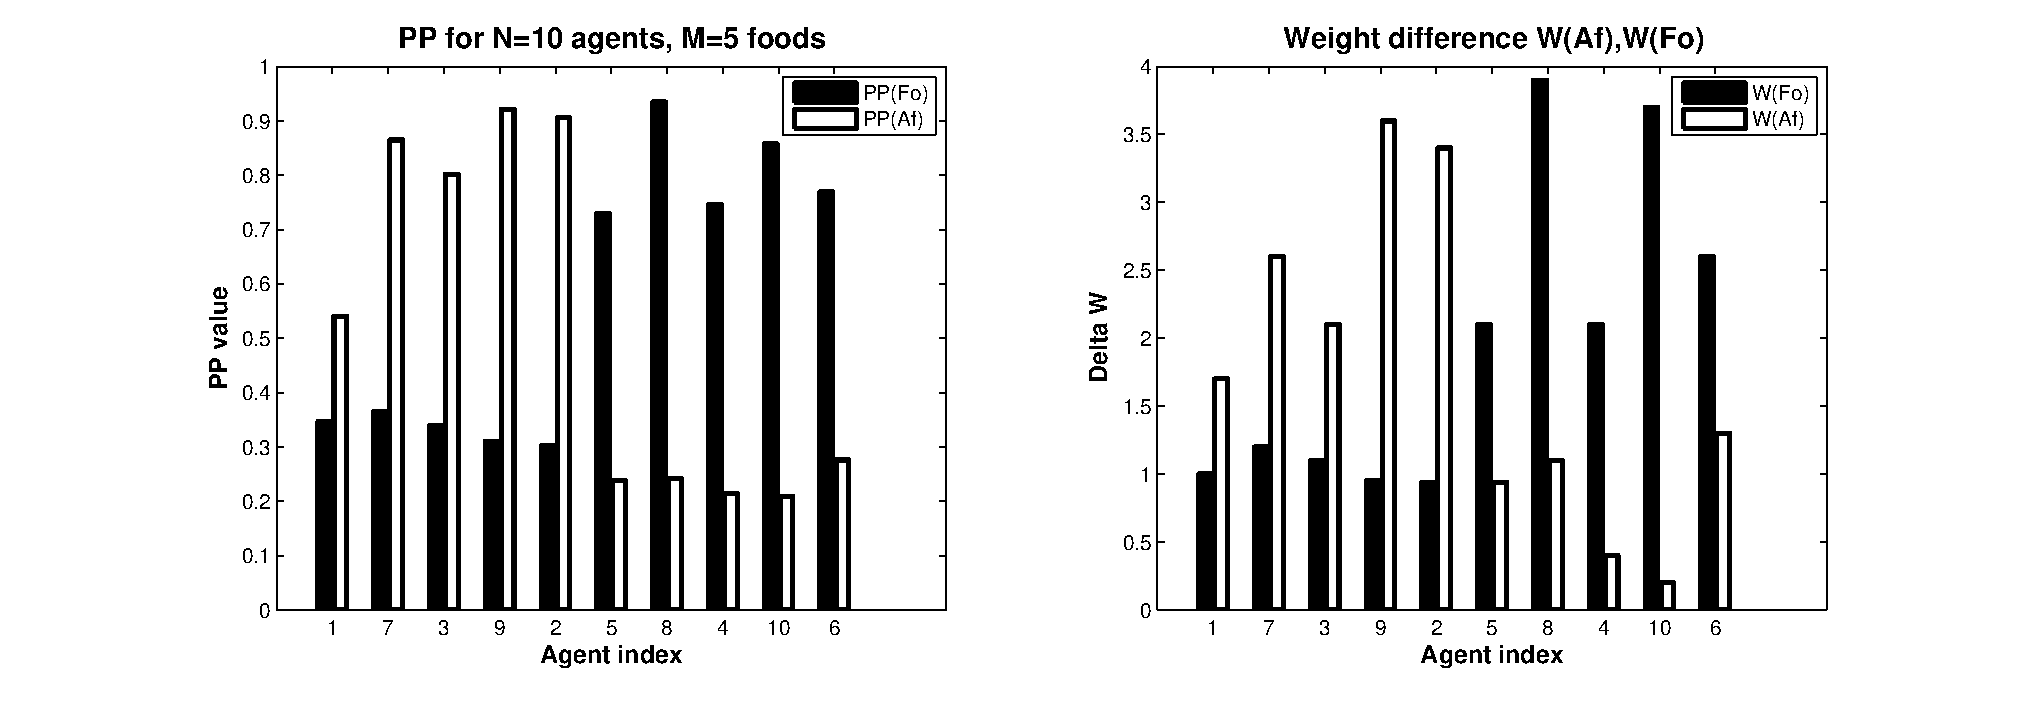
\includegraphics[width=1.0\textwidth]{ppmeasure/social/row1.eps}
        }\\%
        \subfigure[When there are 10 agents and 2 food sources, 2 seekers and 8 parasites are generated]{%
           \label{fig:PPmeasure:social:2}
           \includegraphics[width=1.0\textwidth]{ppmeasure/social/row2.eps}
        }\\ %  ------- End of the first row ----------------------%
        \subfigure[When there are 10 agents and 8 food sources, 8 seekers and 2 parasites are generated]{%
            \label{fig:PPmeasure:social:3}
            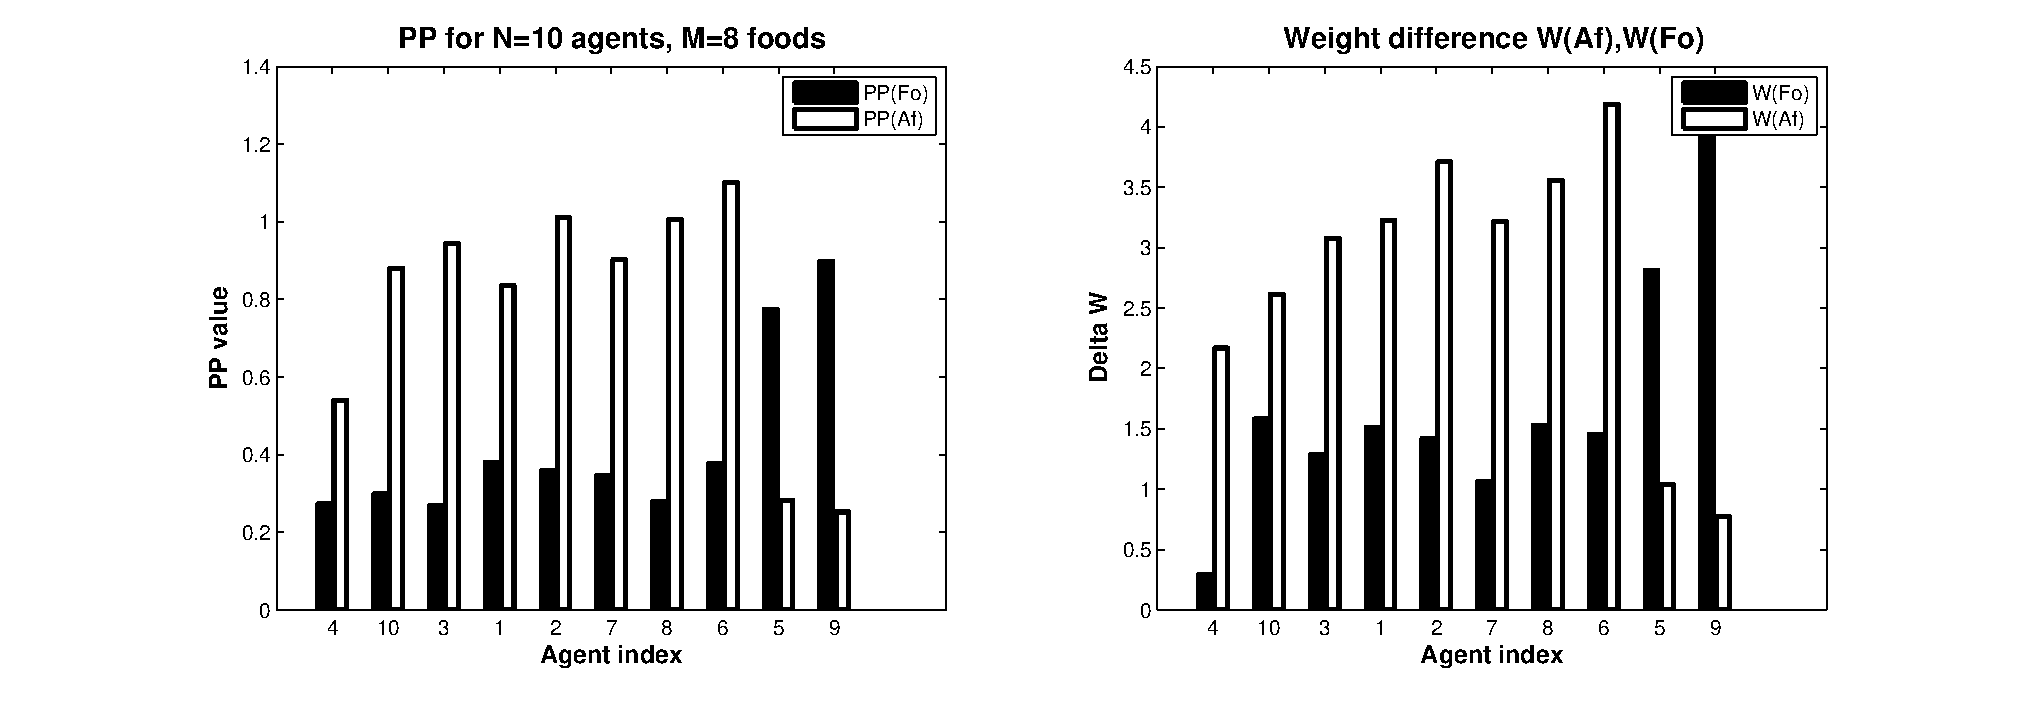
\includegraphics[width=1.0\textwidth]{ppmeasure/social/row3.eps}
        }%
    \end{center}
    \caption{%
     Predictive Measure (PP) computed in the social system for: 
      \textbf{A)} 10 agents and 5 food sources,
      \textbf{B)} 10 agents and 2 food sources,
      \textbf{C)} 10 agents and 8 food sources.
      Left column contains the PP measures with white bars for the food attraction behaviour $PP(Fo)$,
      black bars for the other's attraction behaviour $PP(Af)$.
      Right column contains the weight developed after the system is stabilised for the
      same behaviours $W(Fo),W(Af)$.
    }
\end{figure}

According to this new results, I can state that the weight are an actual
representation of the social division.
However in the future if the developer wants to use more complex agents
in artificial societies, it will be necessary to compute the $PP$ for 
each behaviour and then compare the different behaviours rather then relying exclusively 
on the weight development.

\subsection{Discussion}


In summary, in this study I have analysed an adaptive predictive controller
with the intention to quantify the information used effectively by the robot 
before and after learning.
I introduced the predictive performance to measure the learning ability
of the robot in different tracks.
The robot is facing tracks with increasing difficulty -increasing curvature ratio- 
and is always learning to follow the tracks.
I demonstrated that the predictive performance computed from the agent's 
perspective is consistent with the objective performance on the track.
Additionally I argue that there is a limit in the potential information that an agent can learn,
that enable us to set an upper bound for normalisation purposes.
So the predictive performance help us to measure how much information flow 
the robot is using to achieve its goal without being biased by the absolute weight development.
The predictive performance can be applied to every type of predictive adaptive control 
as long as the predictive and reflex inputs can be identified and is a useful tool 
that can can be used to give an objective estimate of the performance by evaluating information at the subjective level.
The predictive performance is also very useful to determine the performance in the
social system scenario where the highly dynamical setup does not allow the estimation
of an agent performance by looking at the weights.

\subsection{Conlusion final}
The predictive performance was finally applied to the social system scenario
as demonstrated in Section \ref{Chapter8:PPsocial} to show how agents
select either behaviour in terms of information flow.
This analysis show how the agents are selecting the information path and 
how is related to their weights' development.
It also shows that performance cannot be based on the analysis of the weights
but can only be reliably assessed via the predictive performance.